\section{Experimental Results}
\label{experiment}

\subsection{Dataset}
\label{experiment:dataset}
We experiment on four trajectories datasets provided by \cite{ijcai15} that were
extracted from Yahoo! Flickr Creative Commons 100M (a.k.a. YFCC100M) dataset\cite{yfcc100m} 
using photos and videos with geographical locations, timestamps, user identifications etc,
and another trajectories dataset using photos in YFCC100M that were taken in Melbourne,
trajectories were extracted the same way as that described in \cite{ht10, ijcai15},
the time that a user arrived a POI was approximated by the time the first photo taken by that user at that POI,
similarly, the time that a user leaved a POI was approximated by the time the last photo taken by that user at 
that POI \cite{ijcai15}.
An example of trajectory in Melbourne dataset was shown in figure \ref{fig:traj}, 
and statistics of the five datasets are described in table \ref{table:data:all}.


\begin{figure}
\centering
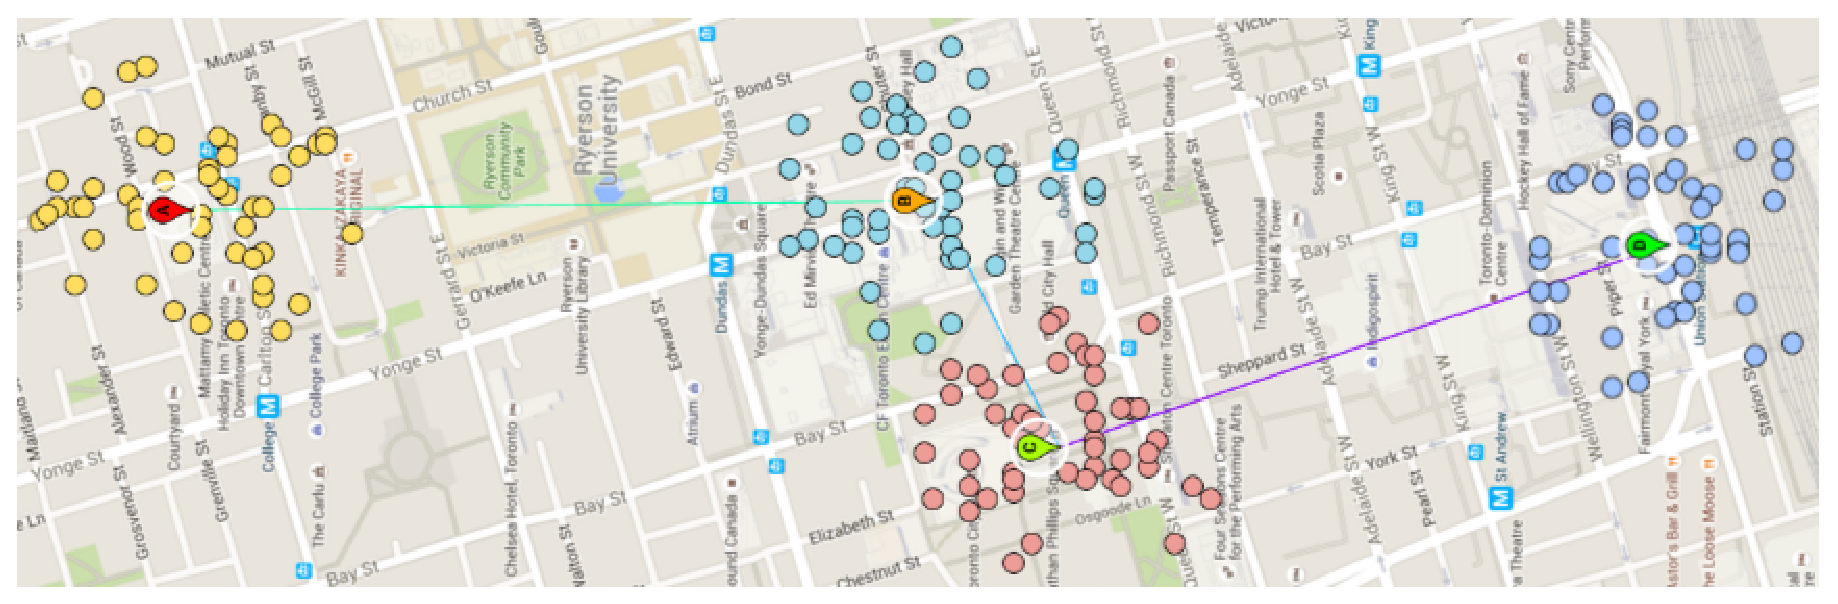
\epsfig{file=traj_eg.eps, width=3.5in}
\caption{An example of trajectory}
\label{fig:traj}
\end{figure}

\begin{table*}
\centering
\caption{Datasets description}
\label{table:data:all}
\begin{tabular}{lrrrrr} \hline
\textbf{Dataset} & \textbf{\#Photos} & \textbf{\#POI Visits} & \textbf{\#Trajectories} & \textbf{\#Users} \\ \hline
Edinburgh & 82,060 & 33,944 & 5,028 & 1,454 \\ 
Glasgow & 29,019 & 11,434 & 2,227 & 601 \\ 
Osaka & 392,420 & 7,747 & 1,115 & 450 \\ 
Toronto & 157,505 & 39,419 & 6,057 & 1,395 \\ 
\hline
\end{tabular}
\end{table*}


\subsection{Evaluation Metrics}
\label{experiment:metric}
We use leave-one-out cross validation to evaluate different trajectory recommendation algorithms,
i.e., when evaluating a specific trajectory of a user, all other trajectories of this user as well as 
all trajectories of other users are used to train the recommendation algorithm.

To evaluate the performance of different trajectory recommendation algorithms,
we employ the trajectory F$_1$-score define in \cite{ijcai15} to measure the POIs that are 
correctly recommended. Let $\mathcal{T}_a$ be the trajectory that was visited in the real world,
and $\mathcal{T}_r$ be the trajectory recommended by one of the algorithms,
trajectory F$_1$-scores was defined as
\begin{displaymath}
    F_1 = \frac{2 |\mathcal{T}_a \cap \mathcal{T}_r|}{|\mathcal{T}_a| + |\mathcal{T}_r|}
\end{displaymath}

In addition, we adapted Kendall's $\tau$ coefficient \cite{kendalltau} to measure the quality of 
recommended visiting order of POIs, which was defined as
\begin{displaymath}
    \tau = \frac{2(N_c - N_d)}{N(N-1)}
\end{displaymath}
where $N_c$ is the number of concordant pairs of POIs in the real visited trajectory $\mathcal{T}_a$ and 
the recommended trajectory $\mathcal{T}_r$, $N_d$ is the number of discordant pairs of POIs in 
$\mathcal{T}_a$ and $\mathcal{T}_r$, $N = |\mathcal{T}_a|$ is the number of visited POIs.


\subsection{Comparison}
% the way to binning POI features, #clusters of POIs,
\label{experiment:comparison}

We compared the experimental results on trajectory datasets between the proposed methods and other 7 methods:
\begin{itemize}
\item \textsc{Random}: choose POIs uniformly at random (without replacement) 
      from the set of POIs $\mathcal{P} \setminus \{p_s, p_e \}$ to visit.
\item \textsc{PersTour}\cite{ijcai15}: personalised trajectory recommendation method described in \cite{ijcai15}, 
      time-based user interest was used and $\eta = 0.5$.
\item \textsc{PersTour-L}: \textsc{PersTour}\cite{ijcai15} with budget constraint replaced with the number POIs to visit, i.e., $L$,
      similar to \textsc{PersTour}, we use time-based user interest and set $\eta$ to $0.5$.
\item \textsc{PoiPopularity}: choose POIs according to the ranking based on POI popularity.
\item \textsc{PoiRank}: choose POIs according to the ranking based on POI features described in section \ref{method:ranking}.
\item \textsc{Markov}: recommend trajectory according to the factorized transition matrix described in section \ref{method:transition},
      using Viterbi algorithm to compute the most likely trajectory w.r.t. constraint $(p_s, p_e, L)$.
\item \textsc{MarkovPath}: the same as Markov, but use integer linear programming to compute the most likely trajectory,
      so that it does not contain self-loops or sub-tours.
\item \textsc{Rank} + \textsc{Markov}: one of the proposed methods, combining POI ranking based on features 
      described in section \ref{method:ranking} and the factorized transition matrix described in section \ref{method:transition},
      use algorithm \ref{dp-algo} to compute the most likely trajectory w.r.t. constraint $(p_s, p_e, L)$.
\item \textsc{Rank} + \textsc{MarkovPath}: the second proposed method, same as Rank + Markov,
      but use integer linear programming to restrict no self-loop or sub-tour appears in the recommended trajectory.
\item \textsc{StructuredSVM}: structured prediction using EdgeFeatureGraphCRF with OneSlackSSVM to recommend trajectory.
\end{itemize}

The F$_1$-scores of different algorithms on five datasets are shown in table \ref{table:f1}
and the values of $\tau$ of different algorithms are show in table \ref{table:tau}
\footnote{We can not compute $\tau$ for \textsc{PersTour} because the number of POIs in recommend trajectory is not guaranteed to equal the number of POIs in real trajectory}.

\subsection{Parameters}
For all algorithms that utilizing ranking probabilities of POIs, namely, \textsc{PoiRank}, \textsc{Rank} + \textsc{Markov} and 
\textsc{Rank} + \textsc{MarkovPath}, the regularization parameter of rankSVM was $10$.
The discretization parameters used to factorize the transition probabilities between POIs was $5$, namely,
either discretizing POI features into $5$ bins in log-space or clustering POIs to $5$ clusters according to the geographical coordinates.
The trade-off parameters $\alpha$ and $\beta$ was set to $0.5$ in both \textsc{Rank} + \textsc{Markov} and 
\textsc{Rank} + \textsc{MarkovPath} algorithms.
The regularization parameter when training \textsc{StructuredSVM} was $1$.


\begin{table*}
\centering
\begin{tabular}{l|cccc} \hline
 & Edinburgh & Glasgow & Osaka & Toronto \\ \hline
\textsc{Random} & $0.571\pm0.139$ & $0.632\pm0.124$ & $0.621\pm0.117$ & $0.621\pm0.128$ \\
\textsc{PersTour}\cite{ijcai15} & $0.656\pm0.223$ & $\mathbf{0.802\pm0.213}$ & $0.702\pm0.230$ & $0.720\pm0.215$ \\
\textsc{PersTour-L} & $0.651\pm0.143$ & $0.660\pm0.102$ & $0.691\pm0.138$ & $0.642\pm0.112$ \\
\textsc{PoiPopularity} & $\mathbf{0.701\pm0.161}$ & $0.745\pm0.166$ & $0.661\pm0.128$ & $0.679\pm0.120$ \\
\textsc{PoiRank} & $0.693\pm0.155$ & $0.777\pm0.169$ & $0.678\pm0.116$ & $\mathbf{0.753\pm0.167}$ \\
\textsc{Markov} & $0.629\pm0.171$ & $0.717\pm0.170$ & $0.679\pm0.162$ & $0.662\pm0.156$ \\
\textsc{MarkovPath} & $0.678\pm0.149$ & $0.735\pm0.170$ & $0.706\pm0.154$ & $0.688\pm0.139$ \\
\textsc{Rank} + \textsc{Markov} & $0.647\pm0.173$ & $0.739\pm0.178$ & $0.705\pm0.171$ & $0.691\pm0.171$ \\
\textsc{Rank} + \textsc{MarkovPath} & $0.688\pm0.154$ & $0.763\pm0.171$ & $\mathbf{0.718\pm0.163}$ & $0.726\pm0.152$ \\
\textsc{StructuredSVM} & - & $0.727\pm0.173$ & $0.715\pm0.170$ & $0.728\pm0.186$ \\
\hline
\end{tabular}
\caption{Performance comparison on four datasets in terms of trajectory F$_1$-score}
\label{table:f1}
\end{table*}



\begin{table*}
\centering
\begin{tabular}{l|cccc} \hline
 & Edinburgh & Glasgow & Osaka & Toronto \\ \hline
\textsc{Random} & $0.259\pm0.156$ & $0.318\pm0.165$ & $0.305\pm0.145$ & $0.309\pm0.166$ \\
\textsc{PersTour-L} & $0.350\pm0.206$ & $0.349\pm0.163$ & $0.415\pm0.243$ & $0.329\pm0.158$ \\
\textsc{PoiPopularity} & $\mathbf{0.422\pm0.257}$ & $0.503\pm0.296$ & $0.361\pm0.194$ & $0.378\pm0.203$ \\
\textsc{PoiRank} & $0.409\pm0.243$ & $\mathbf{0.557\pm0.306}$ & $0.373\pm0.186$ & $0.508\pm0.297$ \\
\textsc{Markov} & $0.404\pm0.229$ & $0.478\pm0.286$ & $0.442\pm0.259$ & $0.404\pm0.229$ \\
\textsc{MarkovPath} & $0.389\pm0.235$ & $0.485\pm0.295$ & $0.445\pm0.268$ & $0.399\pm0.233$ \\
\textsc{Rank} + \textsc{Markov} & $0.420\pm0.244$ & $0.531\pm0.299$ & $0.495\pm0.276$ & $0.451\pm0.264$ \\
\textsc{Rank} + \textsc{MarkovPath} & $0.401\pm0.245$ & $0.531\pm0.309$ & $0.470\pm0.288$ & $0.459\pm0.269$ \\
\textsc{StructuredSVM} & - & $0.505\pm0.282$ & $\mathbf{0.499\pm0.293}$ & $\mathbf{0.511\pm0.312}$ \\
\hline
\end{tabular}
\caption{Performance comparison on four datasets in terms of $\tau$}
\label{table:tau}
\end{table*}


\subsection{Avoid Peeking}
When working with machine learning methods, to make sure the reported performance is a good approximation
of the generalization performance, it is critical to prevent information in test set from leaking into
training set.
Many algorithms in the above comparison utilizing both learning to rank and factorized Markov Chain, 
e.g., \textsc{Rank} + \textsc{Markov}, \textsc{Rank} + \textsc{MarkovPath} and \textsc{StructuredSVM},
both of them need to be trained or parameters be estimated before being used in other algorithms.
Features such as popularity of a POI, the number of visits of a POI and the average visit duration at a POI are
determined by the POI itself as well as trajectories in training set, let's call them aggregated features as they are 
computed by aggregating a set of trajectories.
To make the prediction performance is reliable, it is very important to not include trajectories in test set 
when computing aggregated features.
Unfortunately, it is quite easy, especially when utilizing multiple levels of machine learning models,
to use all data, including those in test set, to compute aggregated features and many researchers and 
practitioners did not realize some bits of information in test set were leaked into training set via these aggregated features.

%One may argue that many of these features will not change much when computed with or without data in test set,
%but in certain areas, such as aerodynamics, some decisions are very sensitive to the quantity of certain features.
%Nevertheless, the exact impact still needs further investigation.

\subsection{Results Analysis}
\begin{table*}
\centering
\begin{tabular}{l|cccccc} \hline
                                    & Query    & POI      & Transition & No sub-tours & Joint    \\ \hline
\textsc{Random}                     & $\times$ & $\times$ & $\times$   & $\times$     & $\times$ \\ 
\textsc{PersTour}\cite{ijcai15}     & $\times$ & $\surd$  & $\times$   & $\surd$      & $\times$ \\
\textsc{PersTour-L}                 & $\times$ & $\surd$  & $\times$   & $\surd$      & $\times$ \\
\textsc{PoiPopularity}              & $\times$ & $\surd$  & $\times$   & $\times$     & $\times$ \\ 
\textsc{PoiRank}                    & $\surd$  & $\surd$  & $\times$   & $\times$     & $\times$ \\
\textsc{Markov}                     & $\times$ & $\surd$  & $\surd$    & $\times$     & $\times$ \\
\textsc{MarkovPath}                 & $\times$ & $\surd$  & $\surd$    & $\surd$      & $\times$ \\
\textsc{Rank} + \textsc{Markov}     & $\surd$  & $\surd$  & $\surd$    & $\times$     & $\times$ \\
\textsc{Rank} + \textsc{MarkovPath} & $\surd$  & $\surd$  & $\surd$    & $\surd$      & $\times$ \\
\textsc{StructuredSVM}              & $\surd$  & $\surd$  & $\surd$    & $\times$     & $\surd$  \\ \hline
\end{tabular}
\caption{Characteristics of different algorithms}
\label{table:character}
\end{table*}
